% slides-graph-dbms-review.tex
% Graph DBMS Review
% Language: Russian
% Author: Evgeny Simonenko <easimonenko@mail.ru>
% License: CC BY-ND 4.0

\documentclass[11pt]{beamer}

\usepackage{polyglossia}
\setdefaultlanguage{russian}
\setotherlanguage{english}
\defaultfontfeatures{Ligatures={TeX},Renderer=Basic}
\setmainfont{FreeSerif}
\setsansfont{FreeSans}
\setmonofont[SizeFeatures={Size=10}]{FreeMono}

\usepackage{graphicx}
\graphicspath{{./images/}}

\title[Графовые СУБД]{Графовые базы данных}
\subtitle{Обзор графовых СУБД}
\author[]{Симоненко Евгений}
\institute[]{Университет ИТМО}
\date[]{Санкт-Петербург, 2022}

\begin{document}

\begin{frame}
  \titlepage
\end{frame}

\begin{frame}
  \frametitle{Содержание}
  \tableofcontents
\end{frame}

\section{Место графовых СУБД в рейтинге}

\begin{frame}
  \frametitle{Топ-10 СУБД}
  DB-Engines Ranking \url{https://db-engines.com/en/ranking}
  \begin{figure}[h!]
    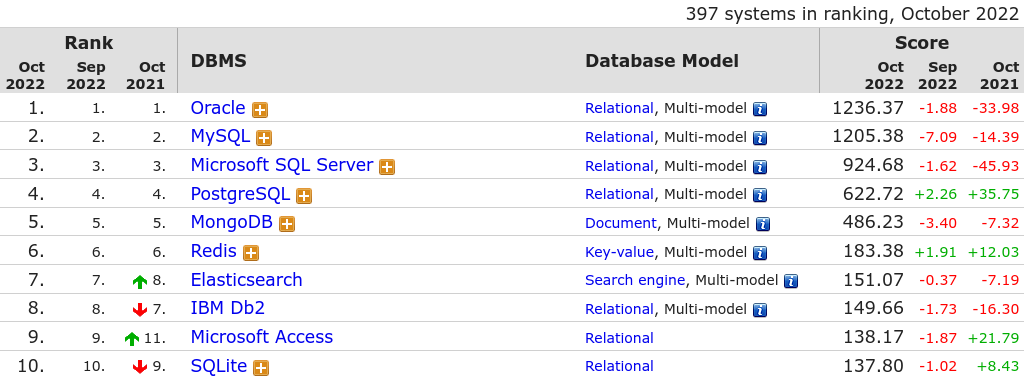
\includegraphics[width=\linewidth]{db-engines_top-10_2022-10-24_14-57-35.png}
  \end{figure}
\end{frame}

\begin{frame}
  \frametitle{Графовые СУБД в общем рейтинге}
  DB-Engines Ranking \url{https://db-engines.com/en/ranking}
  \begin{figure}[h!]
    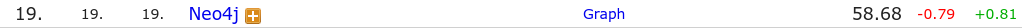
\includegraphics[width=\linewidth]{db-engines_neo4j_2022-10-24_15-39-30.png}
    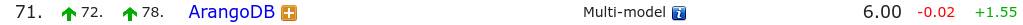
\includegraphics[width=\linewidth]{db-engines_arangodb_2022-10-24_15-40-56.png}
    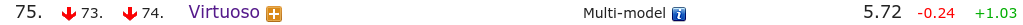
\includegraphics[width=\linewidth]{db-engines_virtuoso_2022-10-24_15-46-33.png}
    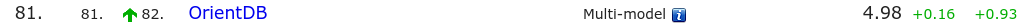
\includegraphics[width=\linewidth]{db-engines_orientdb_2022-10-24_15-45-36.png}
    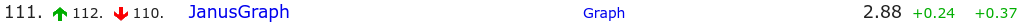
\includegraphics[width=\linewidth]{db-engines_janusgraph_2022-10-24_16-02-48.png}
  \end{figure}
\end{frame}

\begin{frame}
  \frametitle{Топ-20 графовых СУБД}
  DB-Engines Ranking of Graph DBMS \url{https://db-engines.com/en/ranking/graph+dbms}
  \begin{figure}[h!]
    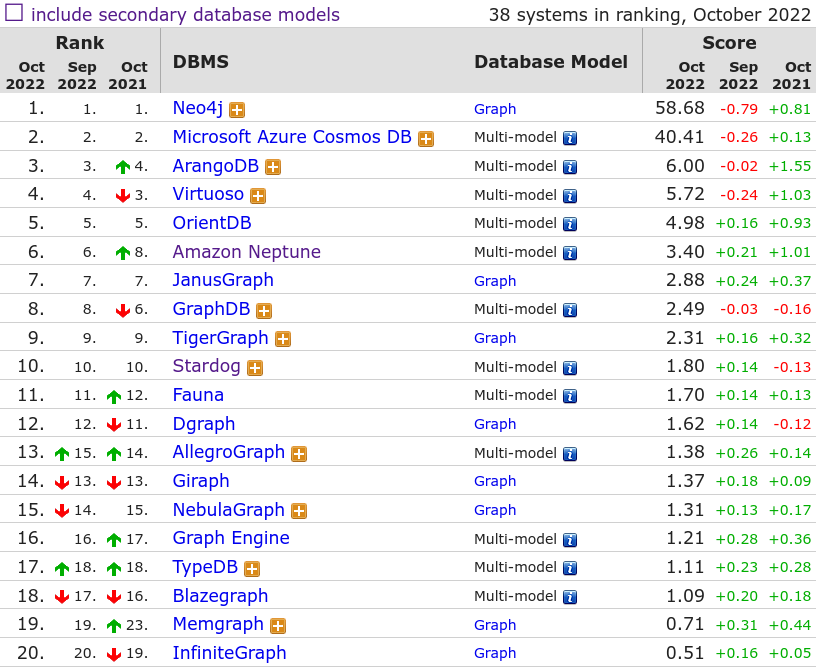
\includegraphics[scale=0.3]{db-engines_top-20-graph-dbms_2022-10-24_15-23-28.png}
  \end{figure}
\end{frame}

\section{Рейтинг СУБД с открытым кодом}

\begin{frame}
  \frametitle{Рейтинг СУБД с открытым кодом}
  \url{https://github.com/easimonenko/research-work/blob/master/graph-databases/graph-databases-short-review.md}
  Топ-5:
  \begin{itemize}
  \item Dgraph -- 18569
  \item Cayley -- 14377
  \item SurrealDB -- 14057
  \item ArangoDB -- 12634
  \item Neo4j -- 10536
  \end{itemize}
\end{frame}

\section{Отличия графовых СУБД друг от друга}

\begin{frame}
  \frametitle{Отличия графовых СУБД друг от друга}
  \begin{itemize}
  \item бывают чисто графовые (Neo4j, JanusGraph), так и мультимодельные (ArangoDB, OrientDB)
  \item имеют разные языки запросов: Cypher (Neo4j, AgensGraph), GraphQL (Dgraph), SQL-подобные (SurrealDB, OrientDB)
  \item реализованы на разных языках программирования: чаще всего на Java, часто на C, C++ и Go
  \item распространяются под разными лицензиями: чаще всего под Apache 2.0, также варианты GNU GPL
  \end{itemize}
\end{frame}

\section*{Благодарность}

\begin{frame}
  \center
  \textit{Благодарю за внимание!}
  
  \textbf{\textsl{\inserttitle}}

  \insertauthor

  \url{mailto:easimonenko@mail.ru}

  \insertinstitute
\end{frame}

\end{document}
